\documentclass[11pt]{article}
\usepackage[margin=1in]{geometry}
\usepackage{amsmath,amssymb}
\usepackage{graphicx}
\usepackage{float}
\usepackage[hidelinks]{hyperref}
\graphicspath{{site_dust/figures/}}
\title{Hard AbsTopK gate after a linear layer on MNIST: hard backward against DUST steps on $W_0$ at four population sizes}
\author{}
\date{2026-10-26}

\begin{document}
\maketitle

\begin{figure}[H]
\centering
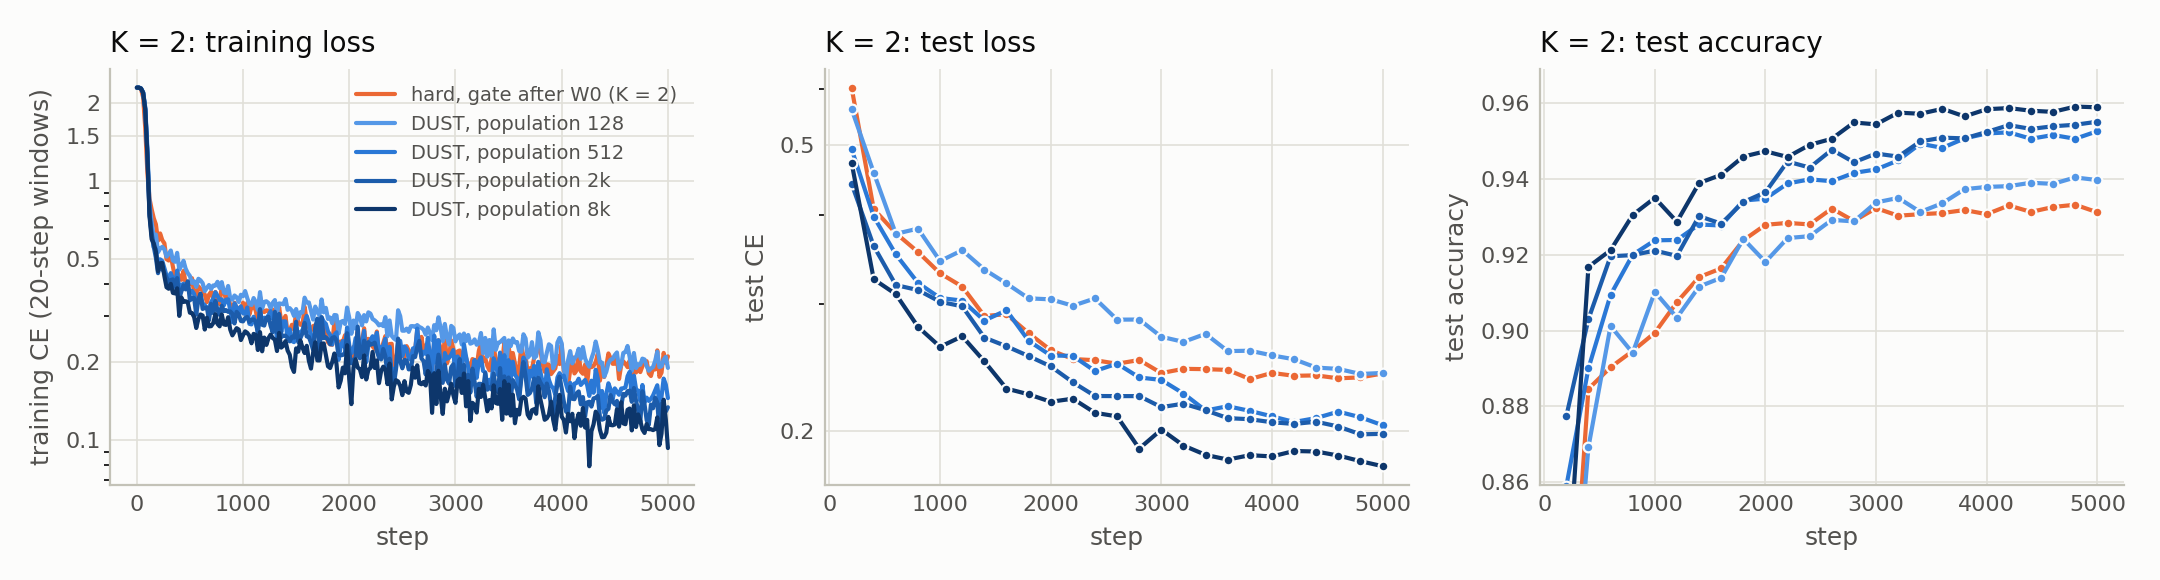
\includegraphics[width=\linewidth]{curves_k2.png}
\caption{$K = 2$: training CE (left, log scale, 20-step window means), test CE (middle, log scale, every 200 steps) and test accuracy (right) for $z = W_2\,\phi(W_1\,\mathrm{AbsTopK}_K(W_0 x))$ trained with the hard backward alone and with every second step a DUST step at population $P \in \{128, 512, 2000, 8000\}$: the gate input $u = W_0 x$ is perturbed on all 784 units with $\mathcal N(0, \sigma^2)$ noise, $\sigma = 0.1$, and the estimate $\hat g_t$ of $\partial L / \partial u_t$ is applied to $W_0$ as $\hat G_{W_0} = \sum_t \hat g_t x_t^\top$. $W_0$ is $784 \times 784$ without bias, hidden width 1024, 5000 steps (2500 hard steps for $W_1, W_2$ in the DUST runs against 5000).}
\label{fig:k2}
\end{figure}

\begin{figure}[H]
\centering
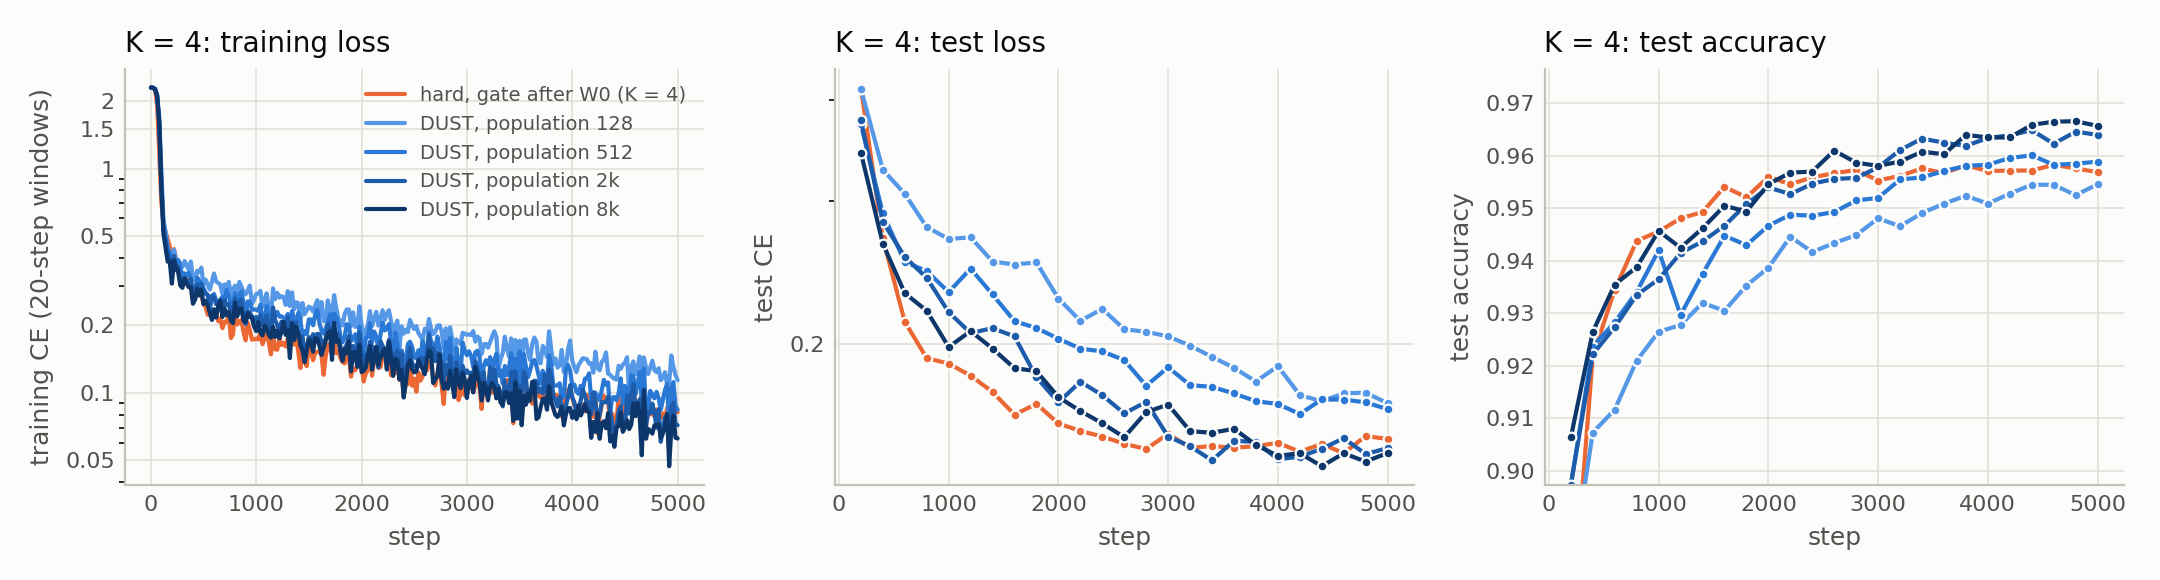
\includegraphics[width=\linewidth]{curves_k4.png}
\caption{$K = 4$: as Figure~\ref{fig:k2}.}
\label{fig:k4}
\end{figure}

\begin{figure}[H]
\centering
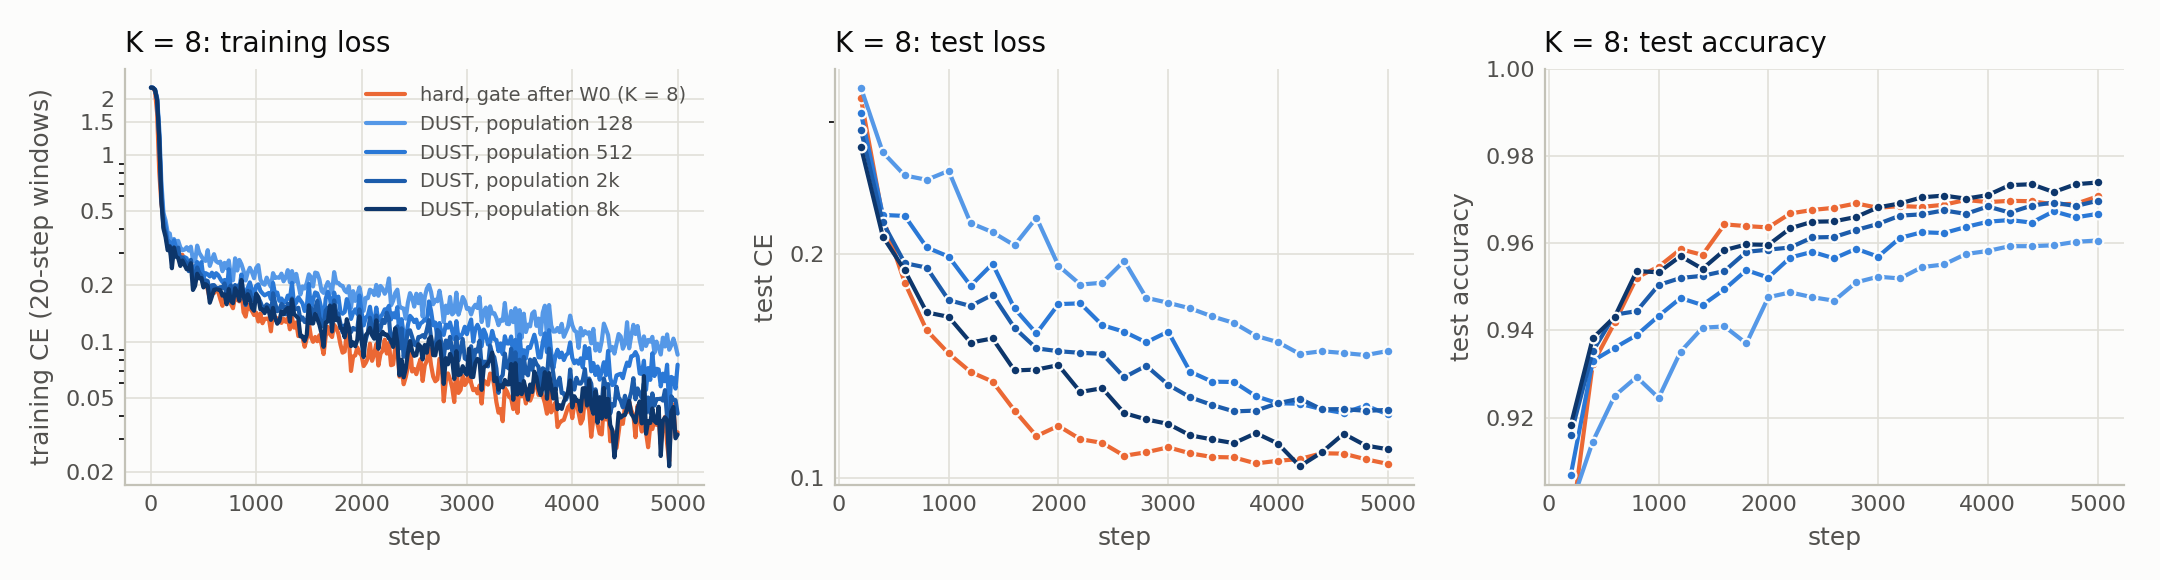
\includegraphics[width=\linewidth]{curves_k8.png}
\caption{$K = 8$: as Figure~\ref{fig:k2}.}
\label{fig:k8}
\end{figure}

\begin{figure}[H]
\centering
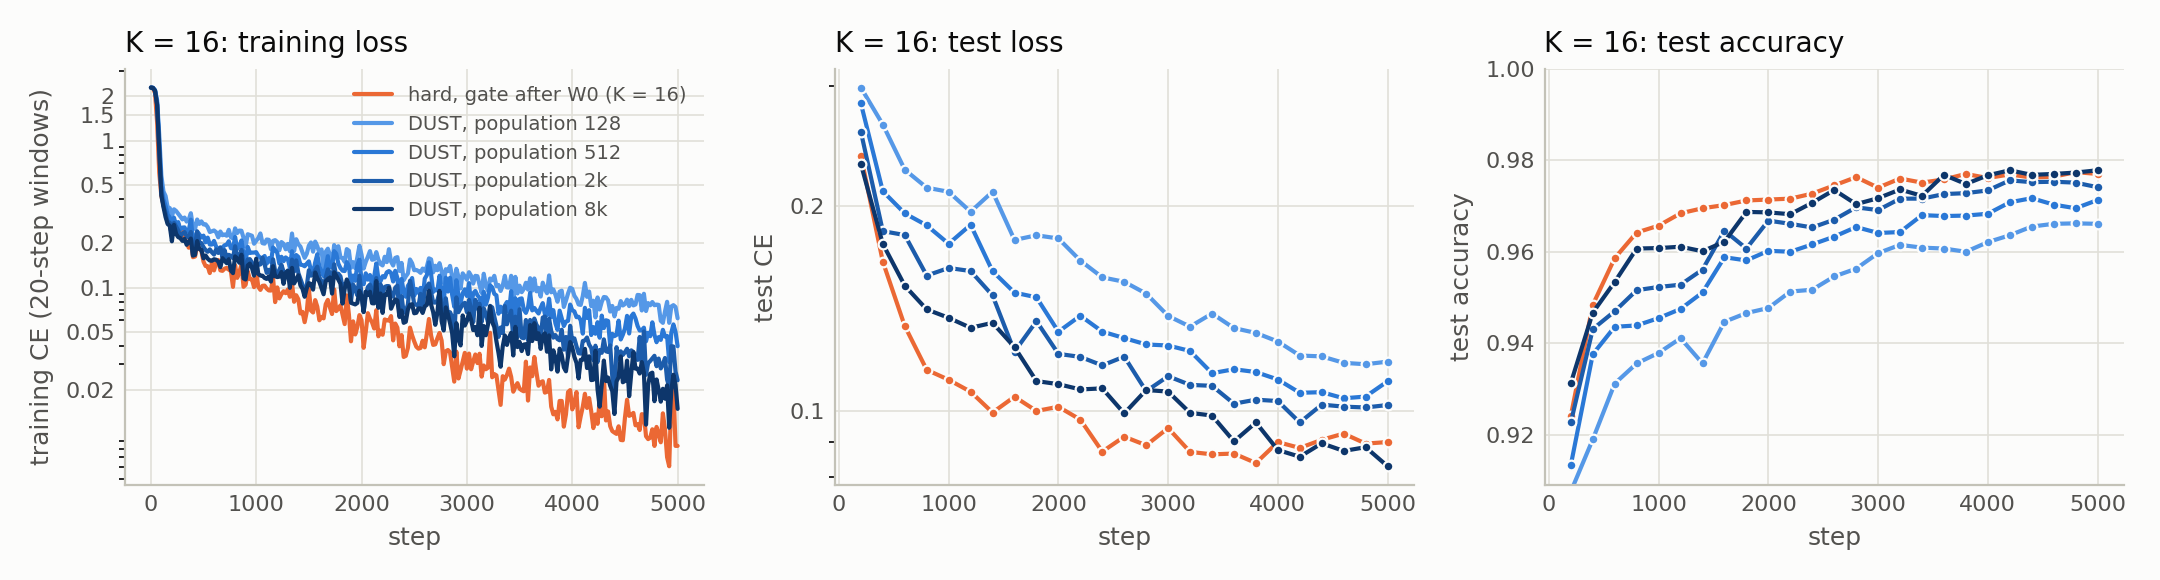
\includegraphics[width=\linewidth]{curves_k16.png}
\caption{$K = 16$: as Figure~\ref{fig:k2}.}
\label{fig:k16}
\end{figure}

\end{document}
